\chapwithtoc{Introduction}
	\ac{TPC} is a~type of gaseous detector that detects charged particle trajectories by measuring the~position and drift time of ions created in the~gas; details are provided in Section~\ref{sec:tpc}. The~energy of such particles can be determined thanks to the~curvature of their trajectory in the~magnetic field.
	
	The~goal of this thesis is to develop an~algorithm for the~reconstruction of charged particle trajectories and energy in an~atypic \ac{TPC} (with orthogonal electric and magnetic fields, i.e., \ac{OFTPC}) used in the~X17 project at the~\ac{IEAPCTU}. Furthermore, we present the~results of testing this algorithm with different samples of simulated data. In the~future, we also plan to test this algorithm by measuring real particles with a~known energy distribution. In order to achieve this, we use the~Garfield++ toolkit~\cite{Garfield++} in combination with the~ROOT~framework~\cite{ROOT}. Some of our more demanding simulations are run on MetaCentrum.
	
	The~X17 project in \ac{IEAPCTU} aims to reproduce measurements of anomalous behavior in the~distribution of angular correlation of pairs produced by the~\ac{IPF} mechanism during the~decay of certain excited nuclei (\iso{Be}{8},~\iso{C}{12},~and~\iso{He}{4}) observed by the~ATOMKI group in Hungary. 
	
	\textcolor{red}{Add citations: MetaCentrum, X17 project, VdG, ATOMKI papers. Maybe also TPC, IPF, etc.}
	
	\section{ATOMKI Measurements}
	\textcolor{red}{Short summary of results of measurements in ATOMKI.}
	
	\section{X17 Project at IEAP CTU}
	\label{sec:IEAP}
		\textcolor{red}{Short summary of our goals, maybe mention the~grant.}
	
		\subsection{Our Detector}
		\textcolor{red}{Short description of our detector. Why we use an~atypic TPC. Gas mixture used in the~detector (70/30) and its effect.}
		
		\subsection{Coordinate System}
			\label{sec:coor}
			\textcolor{red}{Description of the~coordinate system used in this thesis (+ figures). Introduce the~detector space $\mathcal{D}$, the~readout space $\mathcal{R}$ and the~pad space $\mathcal{P}$. TPC dimensions, first sector, pad layout.}
		
			\subsubsection{Detector Space}
				The~detector space $\mathcal{D}$ represents the~physical space of our detector. We describe it using coordinates $(x,y,z)$. The~$z$-axis is the~detector's axis of symmetry, with its positive direction aligned with the~proton beam (\textcolor{red}{or is it opposite? readout has a~negative $z$-coordinate}). The~origin $(0,0,0)$ is located at the~center of the~irradiated target. The~positive $x$-axis passes through the~center of one the~\ac{OFTPC}s along the~intersection of its two planes of symmetry.
				
				Since the~detector has sixfold symmetry, we use only one of its sectors in this work -- the~first sector $\mathcal{D}_1 \subset \mathcal{D}$. This sector contains one of the~six \ac{OFTPC}s and is defined by the~condition:
					\begin{equation}
						(x,y,z) \in \mathcal{D}_1 \Leftrightarrow |y| < x\tan \frac{\pi}{6}.
					\end{equation}
				Simulations in this sector can be applied to all sectors by rotating the coordinates accordingly. The~volume of the~\ac{OFTPC} in this sector, which has the~shape of a~trapezoidal prism, has these boundaries:
					\begin{align}
						x &\in [x_\text{min},x_\text{max}] = [6.51, 14.61] \;\text{cm},\\
						z &\in [z_\text{min},z_\text{max}] = [-8,8] \;\text{cm},\\
						y_\text{max}(x_\text{min}) &= -y_\text{min}(x_\text{min}) =  2.25\;\text{cm},\\
						y_\text{max}(x_\text{max}) &= -y_\text{min}(x_\text{max}) =  7.45\;\text{cm},
					\end{align}
				where $y_\text{max}(x)$ is the~maximal value of the~$y$-coordinate for a~given $x$. The~readout is located at $z = 8$~cm.
			
			\subsubsection{Readout Space}
				The~readout space $\mathcal{R}$ represents the~drift time and final position of ionization electrons as measured by an~ideal continuous readout. We describe it using coordinates $(x',y',t)$, where $x'$ and $y'$ correspond to the~detector coordinates at the readout plane ($z = 8$~cm). 
			
			\subsubsection{Pad Space}
				The~pad space $\mathcal{P}$ represents the~time bin and pad number of ionization electrons as measured by an~ideal discrete readout.
			
				The~readout of the~\ac{OFTPC} will consist (\textcolor{red}{is the design final?}) of 128~rectangular pads arranged in a~staggered pattern (\textcolor{red}{add image where all the parameters are marked}). Most of the~pads are $0.6 \times 0.9$~cm, only pads 102 and 124 are $0.6 \times 0.6$~cm, pad 127 is $0.6 \times 0.509$~cm. The~distance of neighboring pads is 0.08~cm, staggering offset is 0.3946~cm.
	
				\begin{figure}
					\centering
					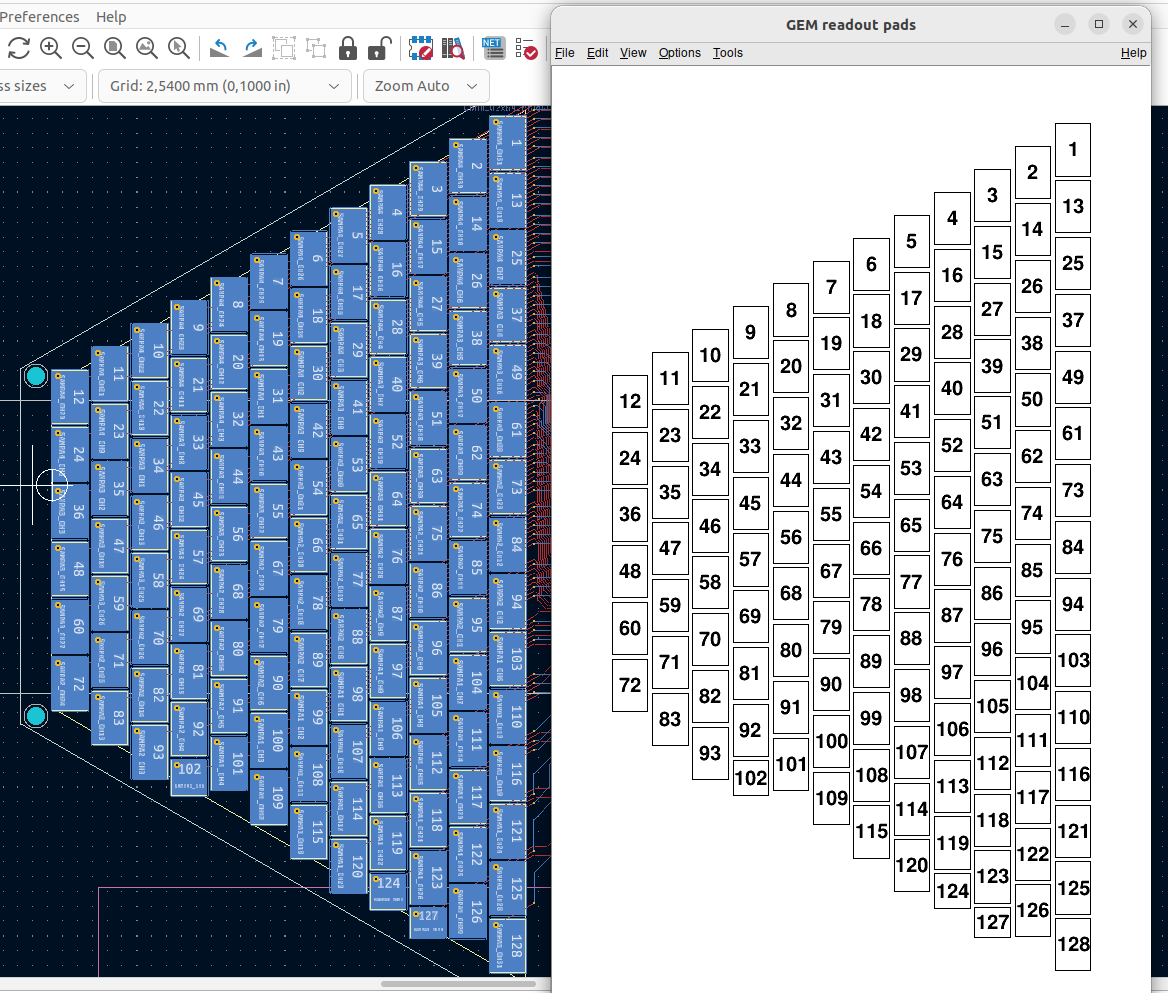
\includegraphics[width=0.8\textwidth]{padlayout.png}
					\caption{Pad layout of the~TPC. \textcolor{red}{Swap for better image.}}
					\label{fig:padlayout}
				\end{figure}
				
		\subsection{Magnetic Field Simulation}
		\textcolor{red}{Magnetic field simulations in Maxwell. Some figures. When working with the~magnetic field outside the~regular grid, we use trilinear interpolation.}
		
			\subsubsection{Trilinear Interpolation}
			\label{sec:trilin}
				Trilinear interpolation is a~generalization of linear interpolation in 3D. It can be used to interpolate a~function whose values are known on a~regular grid. We use this simple method for interpolating the~magnetic field, and it is also used in Section~\ref{sec:grad} to interpolate the~Ionization Electron Map. In both cases, we use a~cubic grid.
				
				Let us consider a~cube (a~cell of our regular grid) with an~edge of length~$a$ containing the~point $C = (x,y,z)$ where we want to interpolate a~function $f\!\!:~\!\!\mathbb{R}^3\,\to\,X$ (\textcolor{red}{it should be better explained what $X$ is}). We know the~values of this function on the~vertices of this cube $C_{ijk} = (x_0+ia,y_0+ja,z_0+ka)$, where $i,j,k \in \{0,1\}$. We also define the~points $C_{ij} = (x,y_0+ia,z_0+ja)$ and $C_i=(x,y,z_0+ia)$. Then the~interpolated value $\widehat{f}(C)$ can be calculated as a~composition of three linear interpolations:
					\begin{equation}
						x_d = \frac{x-x_0}{a},~y_d = \frac{y-y_0}{a},~z_d = \frac{z-z_0}{a},
					\end{equation}
					\begin{alignat}{3}
						\widehat{f}(C_{ij}) &= (1-x_d)f(C_{0ij}) \,&+&\,x_d f(C_{1ij}),\\
						\widehat{f}(C_{i}) &= (1-y_d)\widehat{f}(C_{0i}) &+&\,y_d \widehat{f}(C_{1i}),\\
						\widehat{f}(C) &= (1-z_d)\widehat{f}(C_0) &+&\,z_d \widehat{f}(C_1).
					\end{alignat}
				We can also write
					\begin{eqnarray}
						\widehat{f}(C) = \sum_{i,j,k \in \{0,1\}} t_x^i t_y^j t_z^k f(C_{ijk}),\\
						t_a \stackrel{\text{def}}{=} \begin{pmatrix}t_a^0\\ t_a^1\end{pmatrix} = \begin{pmatrix}1-a_d\\ a_d\end{pmatrix},\quad a \in \{x,y,z\},
					\end{eqnarray}
				or as a~polynomial:
					\begin{equation}
						\widehat{f}(C) = \sum_{a,b,c \in \{0,1\}}\sum^{a}_{i=0}\sum^{b}_{j=0}\sum^{c}_{k=0} (-1)^{(a-i)+(b-j)+(c-k)} f(C_{ijk}) x_d^a y_d^b z_d^c.
					\end{equation}
				%\begin{equation}
				%	\widehat{f}(C) = (1-x_d) (1-y_d) (1-z_d) f(C_{000}) + (1-x_d) (1-y_d) z_d f(C_{001}) + (1-x_d) y_d (1-z_d) f(C_{010}) + (1-x_d) y_d z_d f(C_{011}) + x_d (1-y_d) (1-z_d) f(C_{100}) + x_d (1-y_d) z_d f(C_{101}) + x_d y_d (1-z_d) f(C_{110}) + x_d y_d z_d f(C_{111})
				%\end{equation}
				
				\begin{figure}
					\centering
					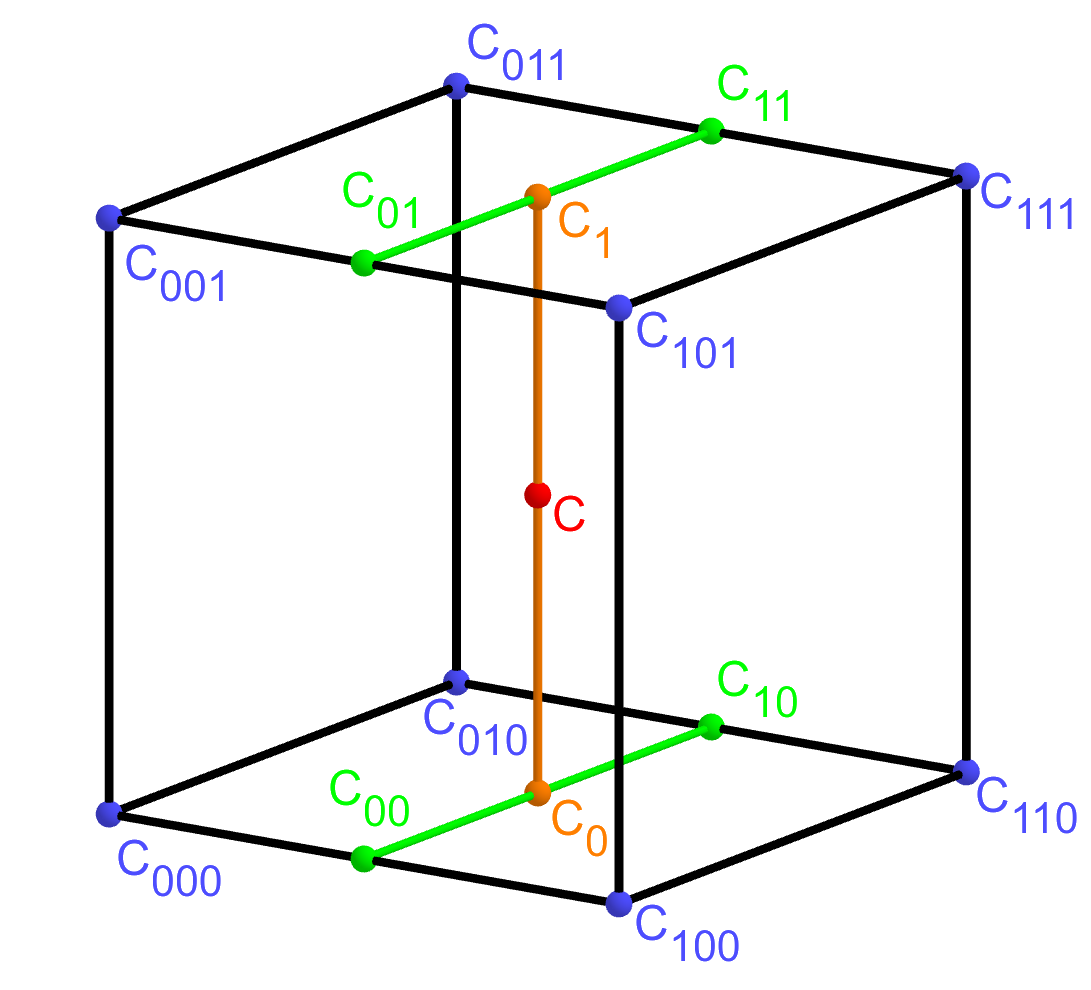
\includegraphics[width=0.5\textwidth]{trilinear.png}
					\label{fig:trilin}
					\caption{Visualization of trilinear interpolation as a~composition of linear interpolations. \textcolor{red}{Image drawn in GeoGebra and inspired by a~similar image on Wikipedia (looks a~bit worse) -- is credit necessary?}}
				\end{figure}
				
				\textcolor{red}{Maybe a~citation here, although I am not sure it is necessary since it could be considered common knowledge. Maybe $x_0$, etc. should be explicitly described.}